\documentclass[a4paper,portrait,columns=2, hidelinks]{cheatsheet}
\usepackage{graphicx}
\usepackage{tikz}
\usetikzlibrary{positioning}
\usetikzlibrary{arrows}
\usetikzlibrary{decorations.pathreplacing}

\usepackage{bbm}
\usepackage{graphicx}
\usepackage{xcolor} % For color
\usepackage{subcaption}
\usepackage{booktabs}

\title{Probability and Statistics}
\author{Matthew Scicluna\\\href{mailto:matthew.scicluna@umontreal.ca}{matthew.scicluna@umontreal.ca}}
\begin{document}

%\maketitle


\section{Probability and Statistics}
\textbf{Probability}: Given Model, how likely is Data? $\rightarrow$ Well-formed since these are Mathematical questions.\\
\textbf{Statistics}: Given Data, how likely is Model? $\rightarrow$ Ill-formed since many Models can generate the same data!

\begin{center}
	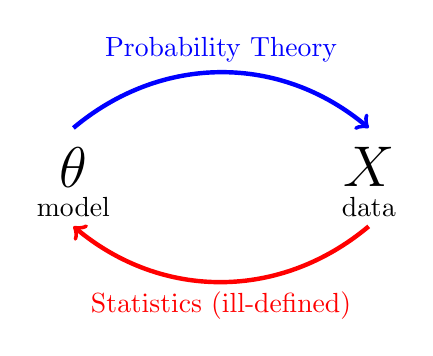
\begin{tikzpicture}[scale=2.5]
	\node [blue] at (0.75, 0.4) {Probability Theory};
	\node [red] at (0.75, -0.9) {Statistics (ill-defined)};
	\draw [->,ultra thick,blue] (0,0) to [bend left=40] (1.5,0);
	\draw [->,ultra thick,red] (1.5,-0.5) to [bend left=40] (0,-0.5) ;
	\node at (0,-0.2) {\huge{$ \theta $}};
	\node at (1.5,-0.2) {\huge{$ X $}};
	\node at (0,-0.4) {model};
	\node at (1.5,-0.4) {data};
	\end{tikzpicture}
\end{center}

There are two interpretations for what the Probability of an Event means:
\begin{enumerate}
	\item \textbf{Frequentists}: \emph{limiting frequency} of the Event
	\item \textbf{Bayesians}: \emph{subjective belief} that the Event occurs
\end{enumerate}

\section{Probability Space}
\textbf{Probability Space}: a triple \( (\Omega, F, P)\) consisting of:
\begin{enumerate}
	\item \( \Omega \) the \textbf{Sample Space}
	\item \( F \subseteq 2^{\Omega}\) a \textbf{\(\sigma\)-algebra}\hyperref[sec:ft1]{$^1$} on \(\Omega\)  i.e.
	\begin{enumerate}
		\item \(\Omega \in F\)
		\item \(E \in F \Rightarrow E^{\complement} \in F\)
		\item \(E_1, E_2, \cdots \in F \Rightarrow\bigcup_{i=1}^{\infty} E_i \in F\)
	\end{enumerate}
	\item \(P\): \(F \mapsto [0,1] \) a \textbf{Probability Measure} i.e.
	\begin{enumerate}
		\item \(P(E) \ge 0\) for \(E \in F\)
		\item \(P(\Omega) = 1\)
		\item \(P \left(\bigsqcup_{i=1}^{\infty} E_i \right)\Rightarrow\sum_{i=1}^{\infty} P(E_i)\) for \(E_i \in F\)
	\end{enumerate}
\end{enumerate}

Given \textbf{Events} \(E_i, E \in F\), $P$ also satisfies:
\begin{enumerate}
\item \textbf{Upward and Downward continuity} of \(P\):
	\begin{enumerate}
	\item \(E_i \uparrow E \Rightarrow \lim\limits_{n\to\infty} P(E_n) = P(E) \)
	\item \(E_i \downarrow E \Rightarrow \lim\limits_{n\to\infty} P(E_n) = P(E) \)
	\end{enumerate}
\item \textbf{Monotonicity} of \(P\):
        \begin{enumerate}
        	\item \( E_i \subseteq E_j \Rightarrow P(E_i) \le P(E_j)\)
        \end{enumerate}
\end{enumerate}

\section{Conditional Probability}
We can compute Probabilities of Events Conditioned on other Events. \\
\textbf{Conditional Probability} of event \(A\) on event \(B\) with \(P(B) > 0\) is:
\begin{align*}
P(A \mid B) = \frac{P(A \cap B)}{P(B)} = \frac{P(B \mid A)P(A)}{P(B)}
\end{align*}

A set of events \(\{A_i\}\) are \textbf{Mutually Independent} if, for any subset of \(\{A_j\}_{j\in k}\):
\begin{align*}
P \left( \bigcap_{j\in k} A_j \right) = \prod_{j\in k}P(A_j) 
\end{align*}

\textbf{Law of Total Probability}: Given Events \(A\) and \textbf{Partition} \(\{B_i\}\) (i.e. where \(\bigsqcup_{i=1}^{\infty} B_i = \Omega \) )
\begin{align*}
P(A) = \sum_{i=1}^{\infty} P(A \mid B_i)P(B_i)
\end{align*}

\section{Random Variables}

A \textbf{Random Variable} is a \(\mathbb{B}\)-Measurable function \\
X: \( (\Omega, F) \mapsto (\mathbb{R},\mathbb{B}) \)\hyperref[sec:ft1]{$^2$}
\begin{enumerate}
	\item For \( A \in \mathbb{B}\) we can compute \( P(X \in A)\)
	\item \( P(X \in A) := P(X^{-1}(A)) = P(\{ \omega \in \Omega : X(\omega) \in A \})\)
	\item \( P(X^{-1}(\cdot)) := P_X(\cdot)\) which is called the \textbf{Push-Forward Measure} of \(P\) by \(X\) on \( \mathbb{R}\)
	\item Hence \( X\) induces a new Probability Space \((\mathbb{R}, \mathbb{B}, P_X) \) from the original \( (\Omega, F, P)\)
\end{enumerate}

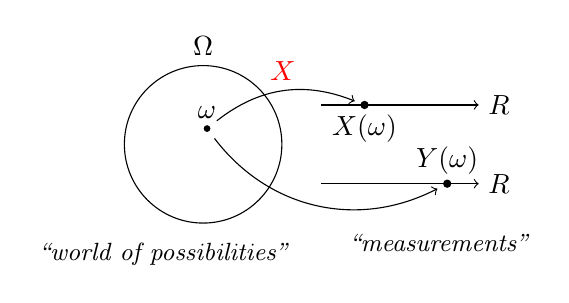
\begin{tikzpicture}[scale=0.5]
%% \draw[help lines] (0,0) grid (12,6);
%% \node [align=center, red] at (1, 1.5) {bla \\ bla} ;
%% \draw [blue, thick] (6,5) rectangle (10,10);
\draw (0,0) circle (2cm);
\node[above] at (0,2) {$\Omega$};
\node (o) at (0.1,.4) {};
\draw (o) circle[radius=2pt] node[above] {$\omega$};
\fill (o) circle[radius=2pt];
\node at (-1,-2.8) {\emph{\small ``world of possibilities''}};

\draw [->] (3,1) -- (7,1) node[right]{$\mathbb{R}$};
\node (x) at (4.1,1) {};
\draw (x) circle[radius=2pt] node[below] {$X(\omega)$};
\fill (x) circle[radius=3pt];
\draw [->, black!70!black] (o) to [bend left=30] node[midway, above, red] {$X$} (x);

\draw [->] (3,-1) -- (7,-1) node[right]{$\mathbb{R}$};
\node (y) at (6.2,-1) {};
\draw (y) circle[radius=2pt] node[above] {$Y(\omega)$};
\fill (y) circle[radius=3pt];
\draw [->, thin] (o) to [bend right=40] (y);
\node at (6,-2.5) {\emph{\small ``measurements''}};
\end{tikzpicture}

Random Variables can be uniquely determined by their \textbf{CDF}:
\( F_X(t) := P_X\left((-\infty,t]\right) = P(X \le t) \)
\begin{enumerate}
	\item Right Continuous
	\item Non-Negative
	\item \(\lim\limits_{t \to \infty} F_X(t) = 1, \lim\limits_{t \to -\infty} F_X(t) = 0\)
\end{enumerate}
Any function satisfying above properties is the CDF for some random variable.

\hfill

Random Variables studied are usually either \textbf{Continuous} or \textbf{Discrete} (they can also be \textbf{Singular} or \textbf{Mixed}).
\begin{enumerate}
	\item If \( F_X\) \textbf{Absolutely Continuous} then \(X\) is a Continuous RV.\hyperref[sec:ft3]{$^3$}
	\begin{enumerate}
		\item \textbf{Absolutely Continuous}: $F$ differentiable a.e. and $\exists f(x)$ s.t. $F_X(x) = \int_{-\infty}^{x} f(u) du$
		\item $\Rightarrow$ $\frac{d}{dx}F_X(x) = f(x)$ wherever $F$ is differentiable
		\item \(f\) is called the \textbf{PDF}
		\item $f$ is unique a.e. (may not be everywhere!)
		\item If \(X\) also Non-Negative then \textbf{Hazard} of X is \( \lambda(t) = \frac{f(t)}{1 - F(t)}\)	
		\begin{enumerate}
			\item \(1 - F(t) = \exp\left(-\int_0^t \lambda(x)\,dx \right) \)
			\item \(\lambda(t)\) interpreted as instantaneous survival rate at time t.
			\item \( \lambda(t) = c \ \forall t \iff X \sim Exp(c) \)
		\end{enumerate}
	\end{enumerate}
	\item If \(X(\Omega)\) is countable then \(X\) is Discrete.
	\begin{enumerate}
		\item \(f(x):=P(\{X=x\})\)
		\item analogously, $F_{X}(t) = \sum_{i=0}^{t}f(i)$\hyperref[sec:ft4]{$^4$}
		\item \(f\) is called the \textbf{PMF}
	\end{enumerate}
\end{enumerate}

\newpage

\section{Random Vectors}
\textbf{Joint CDF} for \( \vec{X} = (X_1, X_2, ..., X_n)\) is \(F(t_1,...,t_n)=P(X_1 \le t_1, ..., X_n \le t_n)\)
\begin{enumerate}
	\item  \textbf{Marginal PDF} of \(\vec{X}_{1:p} = (X_{1}, \cdots X_{p})\) is 
	\begin{align*}
	f_{\vec{X}_{1:p}}\left(\vec{u}_{1:p}\right) = \int_{\vec{X}_{(p+1):n}}f_{\vec{X}}\left(\vec{u}_{1:p}, \vec{X}_{(p+1):n}\right)d\vec{X}_{(p+1):n}
	\end{align*}
	\item \textbf{Conditional PDF} on \(\vec{X}_{1:p}\) given \(\vec{X}_{(p+1):n}\) is 
	\begin{align*}
	f_{\vec{X}_{1:p} | \vec{X}_{(p+1):n}}\left(\vec{u}_{1:p}, \vec{u}_{(p+1):n}\right) =\frac{f_{\vec{X}}\left(\vec{u}_{1:p}, \vec{u}_{(p+1):n}\right)}{f_{\vec{X}_{(p+1):n}}\left(\vec{u}_{(p+1):n}\right)}
	\end{align*}
	\item \textbf{kth Order Statistic} \( X_{(k)}\) of \( \vec{X}\) is the kth smallest value
	\begin{enumerate}
		 \item \( f_{X_{(1)}}(u) = \sum_{i=1}^n f_{X_i}(u)\prod_{j \ne i}(1 - F_{X_j}(u))\)
		\item \( f_{X_{(n)}}(u)=\sum_{i=1}^n f_{X_i}(u)\prod_{j \ne i}F_{X_j}(u)\)
	\end{enumerate}
\end{enumerate}


\section{Moments of a Random Variable}
\(\mathbb{E}_X(X^r) := \mathbb{E}(X^r)\) is the textbf{\(r\)th Moment} of \(X\) under the distribution of \(X\)
\begin{enumerate}
	\item \(\mathbb{E}(X) = \int_0^\infty 1 - F_X(t)\,dt - \int_{-\infty}^0 F_X(t)\,dt\)
	\item If \(X\) Continuous, \(\mathbb{E}(X) = \int_{-\infty}^{\infty} t \cdot f_X(t)\,dt\)
	\item \textbf{LOTUS}: \(\mathbb{E}(g(X)) = \int_{-\infty}^{\infty} g(t) \cdot f_X(t)\,dt\)\hyperref[sec:ft5]{$^5$}
	\item Moments need not exist! (i.e. \(E(|X^r|)=\pm\infty\) )
\end{enumerate}
Can generate Moments using the \textbf{MGF} of \(X\): \( M_X(t) = \mathbb{E} \left(\exp(Xt) \right) \), if \( \exists \epsilon >0 \) s.t. \( \forall |t| < \epsilon\),  \(M_X(t) < \infty \)
\begin{enumerate}
	\item \( \exists \epsilon >0 \) s.t. \( \forall |t| < \epsilon\),  \(M_X(t) = M_Y(t) \Rightarrow X\) and \(Y\) have same distribution
	\item \(\mathbb{E}(|X^r|) = \left.\frac{\partial^r}{\partial^r t}M_X(t)\right\rvert_{t=0}\), if \(M_X\) exists.
	\item If \(\{ X_i\}\) independent RVs, then \( M_{\sum X_i} (t) = \prod M_{X_i}(t)\)
\end{enumerate}

Moments most commonly analyzed are:
\begin{enumerate}
	\item \textbf{Mean} of \(X\): \(\mathbb{E}(X):=\mu_X\)
	\item \textbf{Variance} of \(X\): \(Var(X)=\mathbb{E}((X-\mu_{X})^2)=\sigma^2_{X}\)
\end{enumerate}

For random vectors \(\vec{X}\) we have:
\begin{enumerate}
	\item \(\mathbb{E}(\vec{X}) = [\mathbb{E}(X_1), \cdots, \mathbb{E}(X_n)]=\vec{\mu}\)
	\item \(Cov(\vec{X})= \mathbb{E}[(\vec{X}-\vec{\mu})(\vec{X}-\vec{\mu})^\intercal] = \Sigma\)
\end{enumerate}

If \(X\) and \(Y\) are Random Variables on the same Probability Space
\begin{enumerate}
	\item \textbf{Law of Total Expectation}: If \(\mathbb{E}(|X|)<\infty\) \(\mathbb{E}(X)=\mathbb{E}_{Y}(\mathbb{E}_{X \mid Y}(X \mid Y))\)
	\item \textbf{Law of Total Variance}: If \(Var(X)<\infty\)
	\(Var(X)=\mathbb{E}(Var(X \mid Y))+Var(\mathbb{E}(X \mid Y))\)
\end{enumerate}

\section{Parametric Model}
A \textbf{Parametric model} is a family of distributions that is defined by a fixed finite number of parameters\hyperref[sec:ft6]{$^6$}. Formally,
\begin{align*}
 \mathcal{P}_\Theta = \{ p_\theta (\cdot ; \theta) \mid \theta \in \Theta \}
\end{align*}
\begin{enumerate}
	\item  $p_\theta (\cdot ; \theta)$ is a possible density depending on the \textbf{Parameter} $ \theta $, and $\Theta $ is the \textbf{Parameter Space}
	\item Most important Parametric family: \textbf{Normal Distribution}:
	\begin{enumerate}
		\item \(X \sim \mathcal{N}_p(\mu, \Sigma)\) with \(\mu\in\mathbb{R}^p\), \(\Sigma \in \mathbb{R}^{p \times p}\) Symmetric and Positive Definite iff
		\item  \(\forall a \in \mathbb{R}^p\) we have that \(a^\intercal x \sim \mathcal{N}_p(a^\intercal\mu, a^\intercal\Sigma a)\)
		\item If \(\Sigma\) non-singular, \(f(x)={(2\pi)}^{-\frac{p}{2}}|\Sigma|^{-\frac{1}{2}}\exp{ \left\{-\frac{1}{2}(x-\mu)^\intercal\Sigma^{-1}(x-\mu) \right\} } \)
	\end{enumerate}
	\item Another important family: \textbf{Multinoulli Distribution}
	\begin{enumerate}
		\item $X$ is a discrete RV over $K$ choices.We encode $X$ as a \textbf{one-hot encoding}: a random vector taking values in the unit bases in $\mathbb{R}^{K}$.
		
		\item i.e. \(X(\Omega) = \left\{e_{1}, e_{2}, \ldots, e_{K}\right\}\) where \(e_{j} = \left(0\,\ldots\tikz[remember picture,baseline]{\node[anchor=base] (one-hot-1) {$1$};}\ldots\,0\right)^{T} \in \mathbb{R}^{K}\)
		\tikz[overlay,remember picture]{\draw[stealth'-] (one-hot-1) -- ++(270:0.6cm) -- ++(0:1cm) node[anchor=west,inner ysep=0pt,yshift=1pt] {\scriptsize $j$\textsuperscript{th} coordinate};}
		
		\hfill
		
		\item  $\Theta = \Delta_{K}$ is the \textbf{Probability Simplex} on $K$ choices, and is given by: \(\Delta_{K} = \left\{\pi \in \mathbb{R}^{K}\ ;\ \forall j\ \pi_{j} \geq 0 \text{ and } \sum_{j=1}^{K}\pi_{j} = 1\right\}\)
		\item \(f(x) = p(x;\pi) = \prod_{j=1}^{K}\pi_{j}^{x_{j}}\) where \(x_{j} \in \left\{0,1\right\}\) is the $j$\textsuperscript{th} component of $x$
	\end{enumerate}
	\item From this we get the: \textbf{Multinomial Distribution}
	\begin{enumerate}
		\item \(X = \sum_{i=1}^{n}X_{i}\) where each \(X_i\) are IID multinoulli with same parameter \(\pi\).
		\item \(X(\Omega) = \left\{(n_{1},\ldots,n_{K})\ ;\ \forall j\ n_{j} \in \mathbb{N} \text{ and } \sum_{j=1}^{K}n_{j} = n\right\}\)
	\end{enumerate}
\end{enumerate}

\section{Statistical Decision Theory}

A general theory for using Statistics to make decisions under uncertainty. Specifically, given data \(D \in \mathcal{D}\), \(D \sim P\) for \(P\in \mathcal{P}\)\hyperref[sec:ft7]{$^7$} and set of possible actions \(\mathcal{A}\). Note: \(\Theta\) can be used as \(\mathcal{P}\) if using a Parametric family, in which case \(P := P_{\theta}\).
 \begin{enumerate}
 	\item Our \textbf{Decision Rule} is represented by \(\delta: \mathcal{D} \mapsto \mathcal{A}\)
 	\item The \textbf{Loss} (cost) of doing an action is given by \(L: \mathcal{P} \times \mathcal{A} \mapsto \mathbb{R}\)
 	\item To compare different \(\delta\)'s, can look at the (Frequentist) \textbf{Risk} \(R(P,\delta)=E_{D\sim P}[L(P,\delta(D))]\). Problem: Risk of any \(\delta\) changes with \(P\), so must account for this unless \(\delta\) is Admissible.
 	\begin{enumerate}
	 	\item \(\delta_1\) \textbf{Dominates} \(\delta_2\) (for given loss function \(L\)) if $$R(P,\delta_1)\leq R(P,\delta_2) \forall P \in \mathcal{P}\ and$$
	 	$$\exists P \in \mathcal{P},\ R(P,\delta_1) < R(P, \delta_2)$$
	 	\item We say that a decision rule $\delta$ is \textbf{Admissible} if $\nexists \delta_0$ s.t. $\delta_0$ dominates $\delta$. 
	\end{enumerate}
	\item If no \(\delta\) is Admissible must use a critereon to decide on the optimal one. For Parametric Models:
 	\begin{enumerate}
 		\item \textbf{Minimax Criteria}: Optimal \(\delta\) minimizes Risk in worst case scenerio 
 		$$\delta_{minimax} = \,\min\limits_{\delta}\,\max\limits_{P \in \mathcal{P}}\ R(P,\delta)$$
 		\item Add a \textbf{Weighting} \(\pi\) over $\Theta$ (can be interpreted as a Prior)
 		$$\delta_{weight}= \text{arg}\,\min\limits_{\delta}\,\int_{\Theta}^{}R(P_\theta,\delta)\pi(\theta)d\theta$$
 		\item \textbf{Bayesian Statistical Decision Theory}: Minimize
 		$$\delta_{bayes}(D)= \text{arg}\,\min\limits_{\delta}\,R_B(\delta|D)$$ where $R_B(\delta|D) = \int_{\Theta}^{}L(P_{\theta},\delta)p(\theta|D)d\theta$
 		\begin{enumerate}
 			\item $p(\theta|D)$ is the posterior for a given prior $\pi(\theta)$.
 			\item \(\delta\) chosen this way is optimal for the given \(D\), since any uncertainty (\(\theta\)) is integrated out!
 			\item \(\delta_{bayes}=\delta_{weight}\) if we set \(\pi\) as the prior for \(\Theta\).
 		\end{enumerate}
 	\end{enumerate}
\end{enumerate}

\section{Maximum Likelihood Estimation}
Given some data $x_1, \cdots, x_n$. We want to infer the model which generated the data.

\textbf{Likelihood Function} for some IID observations , coming from a Parametric model is denoted as $\mathcal{L}(\theta)$:
\begin{align*}
\mathcal{L}(\theta) = p(x_{1},\ldots,x_{n};\theta) = \prod_{i=1}^{n}p(x_{i};\theta)
\end{align*}

\section{Bayesian Statistics}

The Bayesian approach is very simple philosophically: it treats all uncertain quantities as random variables.
$$ p(\theta \mid X = x) = \frac{p(x \mid \theta) p(\theta)}{p(x)} $$
where,
\begin{itemize}
	\item[] $ p(\theta \mid X = x) $ is the \emph{posterior belief}, 
	\item[] $ p(x \mid \theta) $ is the \emph{likelihood} or the observation model, 
	\item[] $ p(\theta) $ is the \emph{prior belief} and 
	\item[] $ p(x) $ is the \emph{normalization} or ''marginal likelihood''
\end{itemize}

%	\begin{table*}
%		\caption {Common Parametric Families} \label{tab:title} 
%		\begin{center}		
%			\begin{tabular}{*8l}   
%				\toprule
%			Family & \(p(x \mid \theta)\) & \(\mu_X\)& \(\sigma^2_{X}\)& \(X(\Omega)\)& \(\Theta\) & Notes \\\midrule
%			Multinoulli & \(\prod_{j=1}^{K}\theta_j^{x_j}\) & \(\theta \) & \(\theta(1-\theta) \) & \(\{1, \cdots, k\}\)& \(\Delta_k\)& \\ 
%			Multinomial	&  &  &  \\
%				&  &  &  \\\bottomrule
%				\hline
%			\end{tabular}
%		\end{center}
%	\end{table*}

\newpage

\section{Notes}
\begin{enumerate}
	\item \label{sec:ft1} For some \(\Omega\) we cannot use \(2^{\Omega}\) as a \(\sigma\)-algebra since this may contain sets which do not satisfy all of the axioms. See \cite{Rosenthal2006} for an example.
	\item \label{sec:ft2} Where $\mathbb{B}$ is the \textbf{Borel \(\sigma\)-algebra}: the smallest \(\sigma\)-algebra containing all the open intervals. This must contain all intervals of the form \((-\infty, x]\), and since \(X\) measurable \(\Rightarrow\) \(F_X\) guarenteed to exist.
	\item \label{sec:ft3} Continuity of \(X\) as a function on \(\Omega\) has nothing to do with its continuity as a Random Variable (which depends on the absolute continuity of its CDF) \cite{976739}
	\item \label{sec:ft4} For Discrete RVs, taking \(P\) to be the \textbf{Counting Measure} and \(F=2^{\Omega}\), it can be shown that Lebesgue integrals are sums. Throughout this cheatsheet whenever we display integrals the reader can replace these with sums as needed.
	\item \label{sec:ft5} To be explicit, can write \(\mathbb{E}_{X \sim f}[g(x)]=\int g(x)f(x)dx\)
	\item \label{sec:ft6} Note: Models with infinite sized \(\Theta\) are called \textbf{Non Parametric}.
	\item \label{sec:ft7} Often $P$ will describe an IID process, e.g. $D = (X_1,...,X_n)$ where $X_i \overset{iid}\sim P_0$. In this case, the loss is usually written w.r.t $P_0$ instead of $P$.
\end{enumerate}

\bibliography{prob_cs}
\bibliographystyle{ieeetr}



\end{document}